\documentclass[twoside]{book}

% Packages required by doxygen
\usepackage{fixltx2e}
\usepackage{calc}
\usepackage{doxygen}
\usepackage[export]{adjustbox} % also loads graphicx
\usepackage{graphicx}
\usepackage[utf8]{inputenc}
\usepackage{makeidx}
\usepackage{multicol}
\usepackage{multirow}
\PassOptionsToPackage{warn}{textcomp}
\usepackage{textcomp}
\usepackage[nointegrals]{wasysym}
\usepackage[table]{xcolor}

% Font selection
\usepackage[T1]{fontenc}
\usepackage[scaled=.90]{helvet}
\usepackage{courier}
\usepackage{amssymb}
\usepackage{sectsty}
\renewcommand{\familydefault}{\sfdefault}
\allsectionsfont{%
  \fontseries{bc}\selectfont%
  \color{darkgray}%
}
\renewcommand{\DoxyLabelFont}{%
  \fontseries{bc}\selectfont%
  \color{darkgray}%
}
\newcommand{\+}{\discretionary{\mbox{\scriptsize$\hookleftarrow$}}{}{}}

% Page & text layout
\usepackage{geometry}
\geometry{%
  a4paper,%
  top=2.5cm,%
  bottom=2.5cm,%
  left=2.5cm,%
  right=2.5cm%
}
\tolerance=750
\hfuzz=15pt
\hbadness=750
\setlength{\emergencystretch}{15pt}
\setlength{\parindent}{0cm}
\setlength{\parskip}{3ex plus 2ex minus 2ex}
\makeatletter
\renewcommand{\paragraph}{%
  \@startsection{paragraph}{4}{0ex}{-1.0ex}{1.0ex}{%
    \normalfont\normalsize\bfseries\SS@parafont%
  }%
}
\renewcommand{\subparagraph}{%
  \@startsection{subparagraph}{5}{0ex}{-1.0ex}{1.0ex}{%
    \normalfont\normalsize\bfseries\SS@subparafont%
  }%
}
\makeatother

% Headers & footers
\usepackage{fancyhdr}
\pagestyle{fancyplain}
\fancyhead[LE]{\fancyplain{}{\bfseries\thepage}}
\fancyhead[CE]{\fancyplain{}{}}
\fancyhead[RE]{\fancyplain{}{\bfseries\leftmark}}
\fancyhead[LO]{\fancyplain{}{\bfseries\rightmark}}
\fancyhead[CO]{\fancyplain{}{}}
\fancyhead[RO]{\fancyplain{}{\bfseries\thepage}}
\fancyfoot[LE]{\fancyplain{}{}}
\fancyfoot[CE]{\fancyplain{}{}}
\fancyfoot[RE]{\fancyplain{}{\bfseries\scriptsize Generated by Doxygen }}
\fancyfoot[LO]{\fancyplain{}{\bfseries\scriptsize Generated by Doxygen }}
\fancyfoot[CO]{\fancyplain{}{}}
\fancyfoot[RO]{\fancyplain{}{}}
\renewcommand{\footrulewidth}{0.4pt}
\renewcommand{\chaptermark}[1]{%
  \markboth{#1}{}%
}
\renewcommand{\sectionmark}[1]{%
  \markright{\thesection\ #1}%
}

% Indices & bibliography
\usepackage{natbib}
\usepackage[titles]{tocloft}
\setcounter{tocdepth}{3}
\setcounter{secnumdepth}{5}
\makeindex

% Hyperlinks (required, but should be loaded last)
\usepackage{ifpdf}
\ifpdf
  \usepackage[pdftex,pagebackref=true]{hyperref}
\else
  \usepackage[ps2pdf,pagebackref=true]{hyperref}
\fi
\hypersetup{%
  colorlinks=true,%
  linkcolor=blue,%
  citecolor=blue,%
  unicode%
}

% Custom commands
\newcommand{\clearemptydoublepage}{%
  \newpage{\pagestyle{empty}\cleardoublepage}%
}

\usepackage{caption}
\captionsetup{labelsep=space,justification=centering,font={bf},singlelinecheck=off,skip=4pt,position=top}

%===== C O N T E N T S =====

\begin{document}

% Titlepage & ToC
\hypersetup{pageanchor=false,
             bookmarksnumbered=true,
             pdfencoding=unicode
            }
\pagenumbering{roman}
\begin{titlepage}
\vspace*{7cm}
\begin{center}%
{\Large @Stake }\\
\vspace*{1cm}
{\large Generated by Doxygen 1.8.11}\\
\end{center}
\end{titlepage}
\clearemptydoublepage
\tableofcontents
\clearemptydoublepage
\pagenumbering{arabic}
\hypersetup{pageanchor=true}

%--- Begin generated contents ---
\chapter{Hierarchical Index}
\section{Class Hierarchy}
This inheritance list is sorted roughly, but not completely, alphabetically\+:\begin{DoxyCompactList}
\item Game\+Instance\+Behaviour\begin{DoxyCompactList}
\item \contentsline{section}{Audio\+Controller}{\pageref{class_audio_controller}}{}
\item \contentsline{section}{Player\+Manager}{\pageref{class_player_manager}}{}
\item \contentsline{section}{Score\+Manager}{\pageref{class_score_manager}}{}
\end{DoxyCompactList}
\item Mono\+Behaviour\begin{DoxyCompactList}
\item \contentsline{section}{Audio\+Manager}{\pageref{class_audio_manager}}{}
\item \contentsline{section}{Empty}{\pageref{class_empty}}{}
\item \contentsline{section}{Scene\+Manager}{\pageref{class_scene_manager}}{}
\end{DoxyCompactList}
\end{DoxyCompactList}

\chapter{Class Index}
\section{Class List}
Here are the classes, structs, unions and interfaces with brief descriptions\+:\begin{DoxyCompactList}
\item\contentsline{section}{\hyperlink{class_audio_controller}{Audio\+Controller} }{\pageref{class_audio_controller}}{}
\item\contentsline{section}{\hyperlink{class_audio_manager}{Audio\+Manager} \\*Plays audio clips }{\pageref{class_audio_manager}}{}
\item\contentsline{section}{\hyperlink{class_empty}{Empty} }{\pageref{class_empty}}{}
\item\contentsline{section}{\hyperlink{class_player_manager}{Player\+Manager} \\*Keeps track of all the players in the game. }{\pageref{class_player_manager}}{}
\item\contentsline{section}{\hyperlink{class_scene_manager}{Scene\+Manager} }{\pageref{class_scene_manager}}{}
\item\contentsline{section}{\hyperlink{class_score_manager}{Score\+Manager} \\*Interfaces with Game\+Controller to handle scoring for all players This includes players\textquotesingle{} individual scores and the pot }{\pageref{class_score_manager}}{}
\end{DoxyCompactList}

\chapter{Class Documentation}
\hypertarget{class_audio_controller}{}\section{Audio\+Controller Class Reference}
\label{class_audio_controller}\index{Audio\+Controller@{Audio\+Controller}}
Inheritance diagram for Audio\+Controller\+:\begin{figure}[H]
\begin{center}
\leavevmode
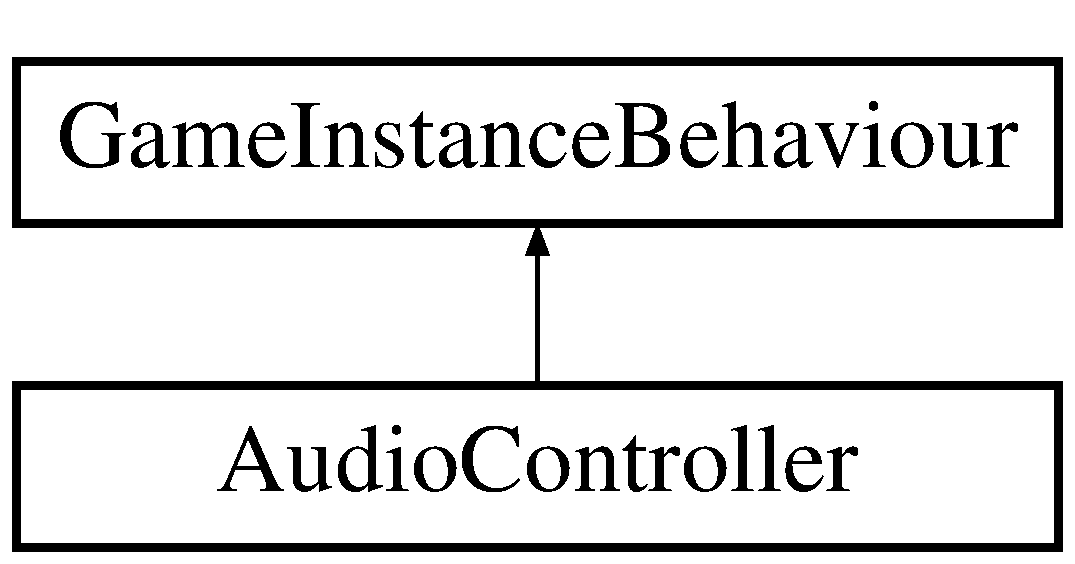
\includegraphics[height=2.000000cm]{class_audio_controller}
\end{center}
\end{figure}
\subsection*{Public Member Functions}
\begin{DoxyCompactItemize}
\item 
void {\bfseries Init} ()\hypertarget{class_audio_controller_aa1241bc01d3057b8ba1fa691d36dd933}{}\label{class_audio_controller_aa1241bc01d3057b8ba1fa691d36dd933}

\item 
void {\bfseries Play} (string clip\+Name)\hypertarget{class_audio_controller_aef70629e0f437c0b9e2113146f17e456}{}\label{class_audio_controller_aef70629e0f437c0b9e2113146f17e456}

\end{DoxyCompactItemize}


The documentation for this class was generated from the following file\+:\begin{DoxyCompactItemize}
\item 
Assets/\+Scripts/Audio\+Controller.\+cs\end{DoxyCompactItemize}

\hypertarget{class_audio_manager}{}\section{Audio\+Manager Class Reference}
\label{class_audio_manager}\index{Audio\+Manager@{Audio\+Manager}}


Plays audio clips  


Inheritance diagram for Audio\+Manager\+:\begin{figure}[H]
\begin{center}
\leavevmode
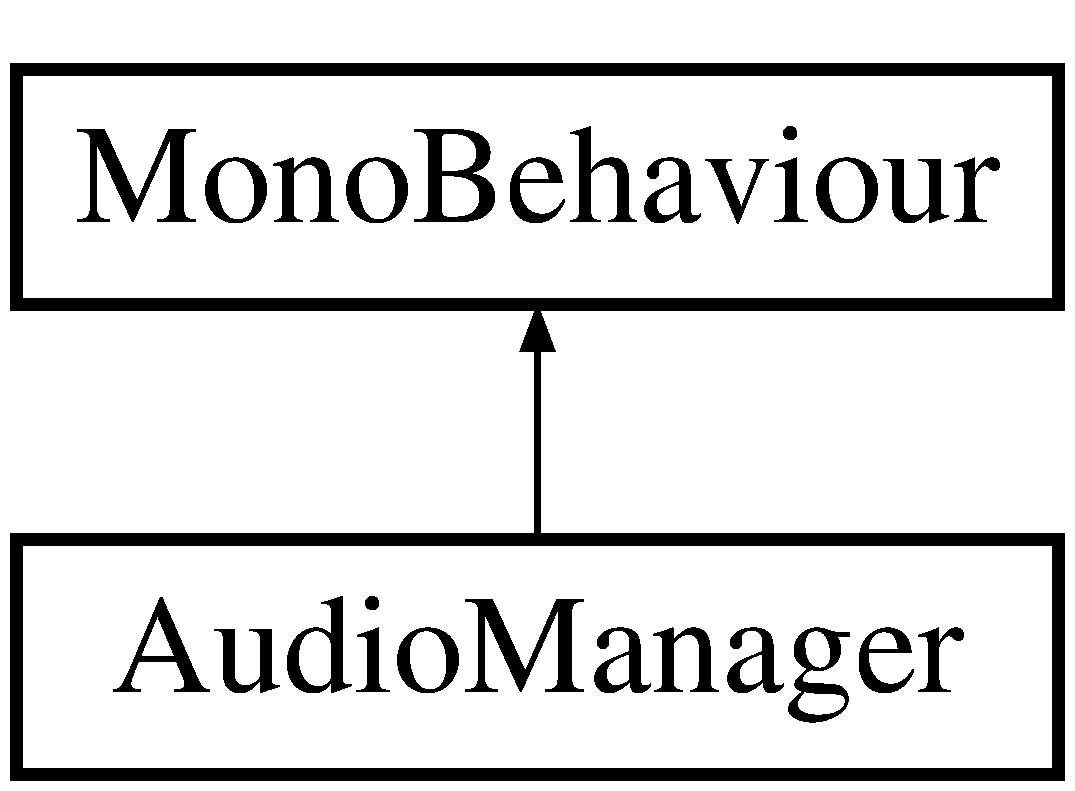
\includegraphics[height=2.000000cm]{class_audio_manager}
\end{center}
\end{figure}
\subsection*{Public Member Functions}
\begin{DoxyCompactItemize}
\item 
void \hyperlink{class_audio_manager_af401954d7711745f75405042bae394a8}{Play} (Audio\+Clip clip)
\begin{DoxyCompactList}\small\item\em Play the audio clip \end{DoxyCompactList}\end{DoxyCompactItemize}
\subsection*{Properties}
\begin{DoxyCompactItemize}
\item 
static \hyperlink{class_audio_manager}{Audio\+Manager} {\bfseries Instance}\hspace{0.3cm}{\ttfamily  \mbox{[}get\mbox{]}}\hypertarget{class_audio_manager_af96f8bc4f9a0ad3f1a63a028bb31f790}{}\label{class_audio_manager_af96f8bc4f9a0ad3f1a63a028bb31f790}

\end{DoxyCompactItemize}


\subsection{Detailed Description}
Plays audio clips 



\subsection{Member Function Documentation}
\index{Audio\+Manager@{Audio\+Manager}!Play@{Play}}
\index{Play@{Play}!Audio\+Manager@{Audio\+Manager}}
\subsubsection[{\texorpdfstring{Play(\+Audio\+Clip clip)}{Play(AudioClip clip)}}]{\setlength{\rightskip}{0pt plus 5cm}void Audio\+Manager.\+Play (
\begin{DoxyParamCaption}
\item[{Audio\+Clip}]{clip}
\end{DoxyParamCaption}
)}\hypertarget{class_audio_manager_af401954d7711745f75405042bae394a8}{}\label{class_audio_manager_af401954d7711745f75405042bae394a8}


Play the audio clip 


\begin{DoxyParams}{Parameters}
{\em clip} & The audio clip to play\\
\hline
\end{DoxyParams}


The documentation for this class was generated from the following file\+:\begin{DoxyCompactItemize}
\item 
Assets/\+Scripts/Audio\+Manager.\+cs\end{DoxyCompactItemize}

\hypertarget{class_empty}{}\section{Empty Class Reference}
\label{class_empty}\index{Empty@{Empty}}
Inheritance diagram for Empty\+:\begin{figure}[H]
\begin{center}
\leavevmode
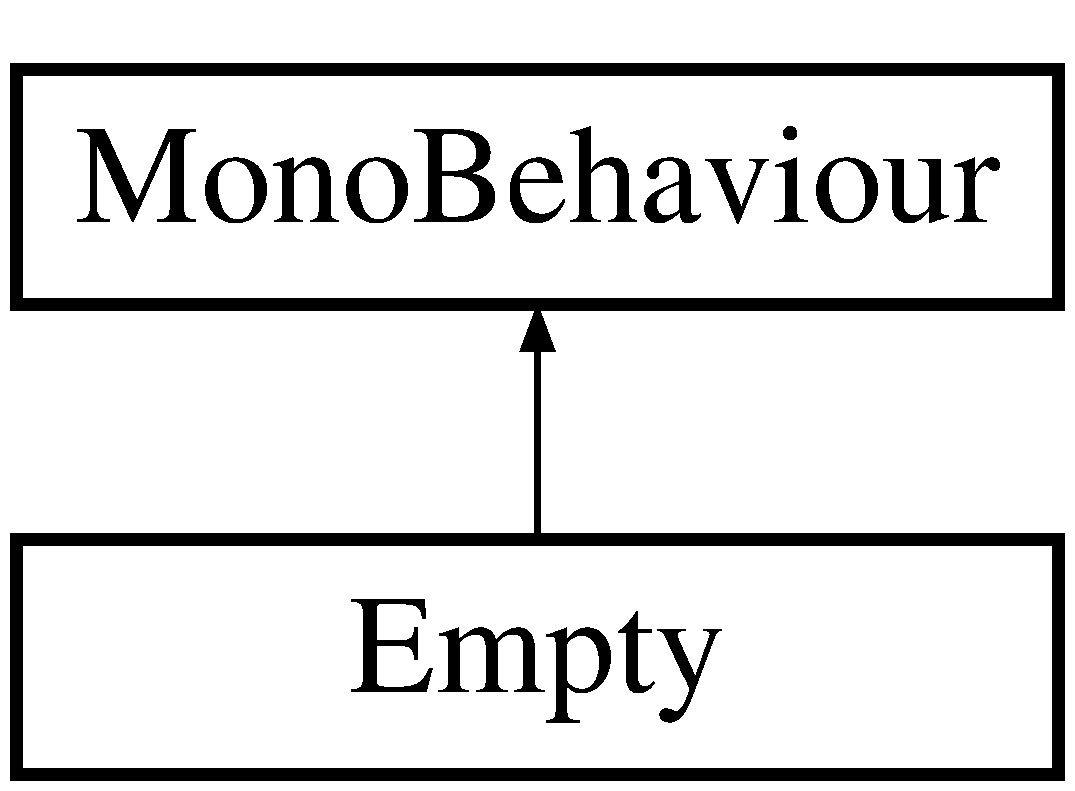
\includegraphics[height=2.000000cm]{class_empty}
\end{center}
\end{figure}


The documentation for this class was generated from the following file\+:\begin{DoxyCompactItemize}
\item 
Assets/\+Scripts/Empty.\+cs\end{DoxyCompactItemize}

\hypertarget{class_player_manager}{}\section{Player\+Manager Class Reference}
\label{class_player_manager}\index{Player\+Manager@{Player\+Manager}}


Keeps track of all the players in the game.  


Inheritance diagram for Player\+Manager\+:\begin{figure}[H]
\begin{center}
\leavevmode
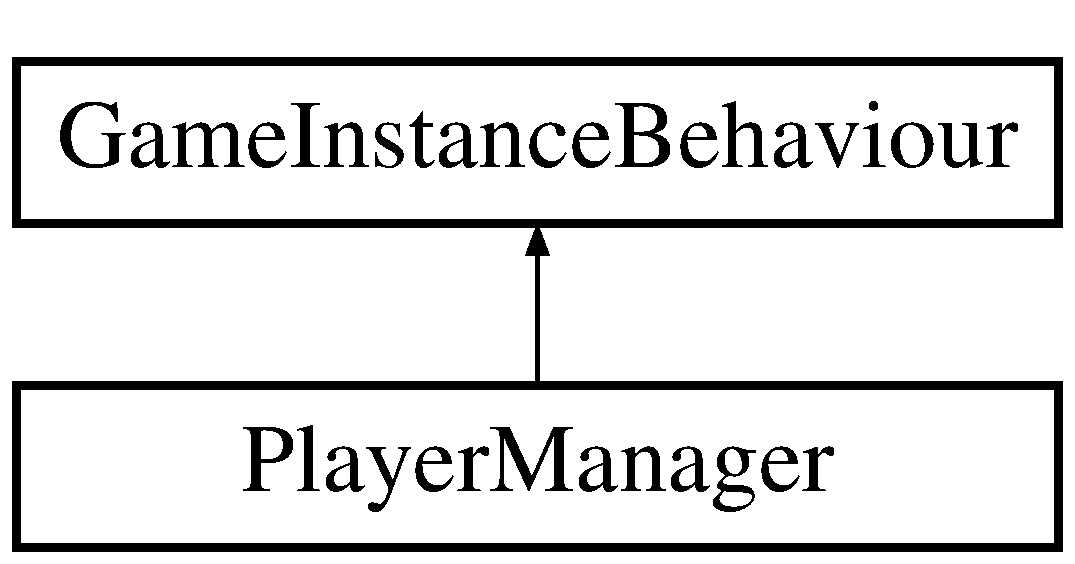
\includegraphics[height=2.000000cm]{class_player_manager}
\end{center}
\end{figure}
\subsection*{Public Member Functions}
\begin{DoxyCompactItemize}
\item 
delegate void {\bfseries On\+Add\+Peer} (string peer, string color)\hypertarget{class_player_manager_a23f484564192af50056793a8beda18ed}{}\label{class_player_manager_a23f484564192af50056793a8beda18ed}

\item 
delegate void {\bfseries On\+Remove\+Peer} (string peer)\hypertarget{class_player_manager_a2ab8d887716b904d65d7d7edacfbdad1}{}\label{class_player_manager_a2ab8d887716b904d65d7d7edacfbdad1}

\item 
void {\bfseries Init} ()\hypertarget{class_player_manager_abd70cd2d0328b9af204cfc4a8a5f2e69}{}\label{class_player_manager_abd70cd2d0328b9af204cfc4a8a5f2e69}

\item 
void {\bfseries Reset} ()\hypertarget{class_player_manager_a413d8be1a89c2428099ea76b74adef08}{}\label{class_player_manager_a413d8be1a89c2428099ea76b74adef08}

\item 
void \hyperlink{class_player_manager_adb5ef6634b1a67bd3a19af09e5cab970}{Add\+Host} (string color)
\begin{DoxyCompactList}\small\item\em Called when the player hosts a new game \end{DoxyCompactList}\item 
void \hyperlink{class_player_manager_affc64e53b2c473f3fc0b4c63756af102}{On\+Update\+Players} (Net\+Message msg)
\begin{DoxyCompactList}\small\item\em Called when a player joins or leaves the room that this player is hosting \end{DoxyCompactList}\end{DoxyCompactItemize}
\subsection*{Public Attributes}
\begin{DoxyCompactItemize}
\item 
On\+Add\+Peer \hyperlink{class_player_manager_a547dd0727a139061c67ffdadd6f8e99c}{on\+Add\+Peer}
\begin{DoxyCompactList}\small\item\em Event that fires when a peer joins the game \end{DoxyCompactList}\item 
On\+Remove\+Peer \hyperlink{class_player_manager_a88f01e2ed833375b7b95ae3d1272baf0}{on\+Remove\+Peer}
\begin{DoxyCompactList}\small\item\em Event that fires when a peer leaves the game \end{DoxyCompactList}\end{DoxyCompactItemize}
\subsection*{Properties}
\begin{DoxyCompactItemize}
\item 
Dictionary$<$ string, Player $>$ \hyperlink{class_player_manager_a6fcc25b412f01d734a22624aa2d3e016}{Players}\hspace{0.3cm}{\ttfamily  \mbox{[}get\mbox{]}}
\begin{DoxyCompactList}\small\item\em Gets the models associated with each player in the game. The key is the player\textquotesingle{}s name. \end{DoxyCompactList}\item 
string \hyperlink{class_player_manager_acf881bd65193d0c3b7089f014ae22057}{Name}\hspace{0.3cm}{\ttfamily  \mbox{[}get, set\mbox{]}}
\begin{DoxyCompactList}\small\item\em Gets/sets this player\textquotesingle{}s name \end{DoxyCompactList}\end{DoxyCompactItemize}


\subsection{Detailed Description}
Keeps track of all the players in the game. 



\subsection{Member Function Documentation}
\index{Player\+Manager@{Player\+Manager}!Add\+Host@{Add\+Host}}
\index{Add\+Host@{Add\+Host}!Player\+Manager@{Player\+Manager}}
\subsubsection[{\texorpdfstring{Add\+Host(string color)}{AddHost(string color)}}]{\setlength{\rightskip}{0pt plus 5cm}void Player\+Manager.\+Add\+Host (
\begin{DoxyParamCaption}
\item[{string}]{color}
\end{DoxyParamCaption}
)}\hypertarget{class_player_manager_adb5ef6634b1a67bd3a19af09e5cab970}{}\label{class_player_manager_adb5ef6634b1a67bd3a19af09e5cab970}


Called when the player hosts a new game 

\index{Player\+Manager@{Player\+Manager}!On\+Update\+Players@{On\+Update\+Players}}
\index{On\+Update\+Players@{On\+Update\+Players}!Player\+Manager@{Player\+Manager}}
\subsubsection[{\texorpdfstring{On\+Update\+Players(\+Net\+Message msg)}{OnUpdatePlayers(NetMessage msg)}}]{\setlength{\rightskip}{0pt plus 5cm}void Player\+Manager.\+On\+Update\+Players (
\begin{DoxyParamCaption}
\item[{Net\+Message}]{msg}
\end{DoxyParamCaption}
)}\hypertarget{class_player_manager_affc64e53b2c473f3fc0b4c63756af102}{}\label{class_player_manager_affc64e53b2c473f3fc0b4c63756af102}


Called when a player joins or leaves the room that this player is hosting 



\subsection{Member Data Documentation}
\index{Player\+Manager@{Player\+Manager}!on\+Add\+Peer@{on\+Add\+Peer}}
\index{on\+Add\+Peer@{on\+Add\+Peer}!Player\+Manager@{Player\+Manager}}
\subsubsection[{\texorpdfstring{on\+Add\+Peer}{onAddPeer}}]{\setlength{\rightskip}{0pt plus 5cm}On\+Add\+Peer Player\+Manager.\+on\+Add\+Peer}\hypertarget{class_player_manager_a547dd0727a139061c67ffdadd6f8e99c}{}\label{class_player_manager_a547dd0727a139061c67ffdadd6f8e99c}


Event that fires when a peer joins the game 

\index{Player\+Manager@{Player\+Manager}!on\+Remove\+Peer@{on\+Remove\+Peer}}
\index{on\+Remove\+Peer@{on\+Remove\+Peer}!Player\+Manager@{Player\+Manager}}
\subsubsection[{\texorpdfstring{on\+Remove\+Peer}{onRemovePeer}}]{\setlength{\rightskip}{0pt plus 5cm}On\+Remove\+Peer Player\+Manager.\+on\+Remove\+Peer}\hypertarget{class_player_manager_a88f01e2ed833375b7b95ae3d1272baf0}{}\label{class_player_manager_a88f01e2ed833375b7b95ae3d1272baf0}


Event that fires when a peer leaves the game 



\subsection{Property Documentation}
\index{Player\+Manager@{Player\+Manager}!Name@{Name}}
\index{Name@{Name}!Player\+Manager@{Player\+Manager}}
\subsubsection[{\texorpdfstring{Name}{Name}}]{\setlength{\rightskip}{0pt plus 5cm}string Player\+Manager.\+Name\hspace{0.3cm}{\ttfamily [get]}, {\ttfamily [set]}}\hypertarget{class_player_manager_acf881bd65193d0c3b7089f014ae22057}{}\label{class_player_manager_acf881bd65193d0c3b7089f014ae22057}


Gets/sets this player\textquotesingle{}s name 

\index{Player\+Manager@{Player\+Manager}!Players@{Players}}
\index{Players@{Players}!Player\+Manager@{Player\+Manager}}
\subsubsection[{\texorpdfstring{Players}{Players}}]{\setlength{\rightskip}{0pt plus 5cm}Dictionary$<$string, Player$>$ Player\+Manager.\+Players\hspace{0.3cm}{\ttfamily [get]}}\hypertarget{class_player_manager_a6fcc25b412f01d734a22624aa2d3e016}{}\label{class_player_manager_a6fcc25b412f01d734a22624aa2d3e016}


Gets the models associated with each player in the game. The key is the player\textquotesingle{}s name. 



The documentation for this class was generated from the following file\+:\begin{DoxyCompactItemize}
\item 
Assets/\+Scripts/Player\+Manager.\+cs\end{DoxyCompactItemize}

\hypertarget{class_scene_manager}{}\section{Scene\+Manager Class Reference}
\label{class_scene_manager}\index{Scene\+Manager@{Scene\+Manager}}
Inheritance diagram for Scene\+Manager\+:\begin{figure}[H]
\begin{center}
\leavevmode
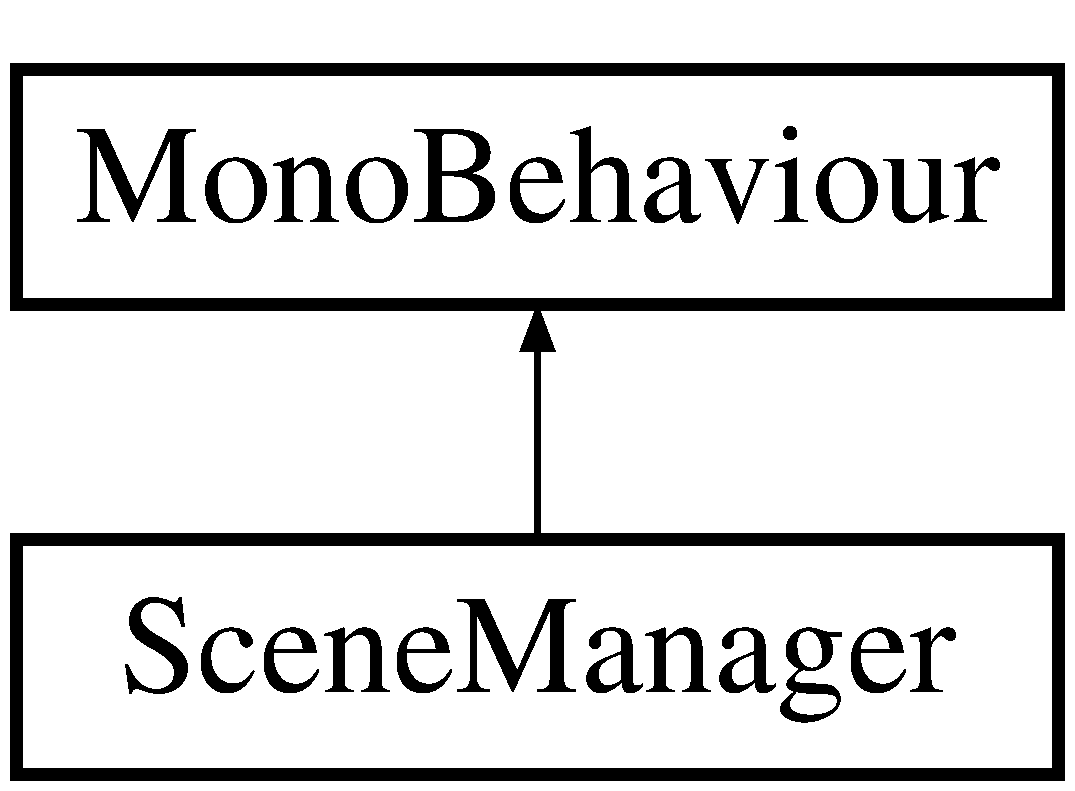
\includegraphics[height=2.000000cm]{class_scene_manager}
\end{center}
\end{figure}
\subsection*{Public Member Functions}
\begin{DoxyCompactItemize}
\item 
void \hyperlink{class_scene_manager_ab402cd27ce43636fedcd3e5fc09eb02c}{Client\+Authenticated} (Dictionary$<$ string, object $>$ response)
\begin{DoxyCompactList}\small\item\em Client was authenticated to A\+PI; we can now get game data and ask player to log in \end{DoxyCompactList}\item 
void \hyperlink{class_scene_manager_a6fd5c1172a1b8501fe96310a8ebd0b34}{User\+Authenticate\+Response} (bool success)
\begin{DoxyCompactList}\small\item\em User attempted authentication; return/show error if failed \end{DoxyCompactList}\end{DoxyCompactItemize}
\subsection*{Public Attributes}
\begin{DoxyCompactItemize}
\item 
string {\bfseries environment}\hypertarget{class_scene_manager_ae8b69f9e6bf2f57497cd6ad69defc83e}{}\label{class_scene_manager_ae8b69f9e6bf2f57497cd6ad69defc83e}

\end{DoxyCompactItemize}


\subsection{Member Function Documentation}
\index{Scene\+Manager@{Scene\+Manager}!Client\+Authenticated@{Client\+Authenticated}}
\index{Client\+Authenticated@{Client\+Authenticated}!Scene\+Manager@{Scene\+Manager}}
\subsubsection[{\texorpdfstring{Client\+Authenticated(\+Dictionary$<$ string, object $>$ response)}{ClientAuthenticated(Dictionary< string, object > response)}}]{\setlength{\rightskip}{0pt plus 5cm}void Scene\+Manager.\+Client\+Authenticated (
\begin{DoxyParamCaption}
\item[{Dictionary$<$ string, object $>$}]{response}
\end{DoxyParamCaption}
)}\hypertarget{class_scene_manager_ab402cd27ce43636fedcd3e5fc09eb02c}{}\label{class_scene_manager_ab402cd27ce43636fedcd3e5fc09eb02c}


Client was authenticated to A\+PI; we can now get game data and ask player to log in 


\begin{DoxyParams}{Parameters}
{\em response} & Dictionary containing \char`\"{}authed\char`\"{} key telling us if A\+PI auth \\
\hline
\end{DoxyParams}
\index{Scene\+Manager@{Scene\+Manager}!User\+Authenticate\+Response@{User\+Authenticate\+Response}}
\index{User\+Authenticate\+Response@{User\+Authenticate\+Response}!Scene\+Manager@{Scene\+Manager}}
\subsubsection[{\texorpdfstring{User\+Authenticate\+Response(bool success)}{UserAuthenticateResponse(bool success)}}]{\setlength{\rightskip}{0pt plus 5cm}void Scene\+Manager.\+User\+Authenticate\+Response (
\begin{DoxyParamCaption}
\item[{bool}]{success}
\end{DoxyParamCaption}
)}\hypertarget{class_scene_manager_a6fd5c1172a1b8501fe96310a8ebd0b34}{}\label{class_scene_manager_a6fd5c1172a1b8501fe96310a8ebd0b34}


User attempted authentication; return/show error if failed 


\begin{DoxyParams}{Parameters}
{\em success} & Was authentication successful?.\\
\hline
\end{DoxyParams}


The documentation for this class was generated from the following file\+:\begin{DoxyCompactItemize}
\item 
Assets/\+Scripts/Scene\+Manager.\+cs\end{DoxyCompactItemize}

\hypertarget{class_score_manager}{}\section{Score\+Manager Class Reference}
\label{class_score_manager}\index{Score\+Manager@{Score\+Manager}}


Interfaces with Game\+Controller to handle scoring for all players This includes players\textquotesingle{} individual scores and the pot  


Inheritance diagram for Score\+Manager\+:\begin{figure}[H]
\begin{center}
\leavevmode
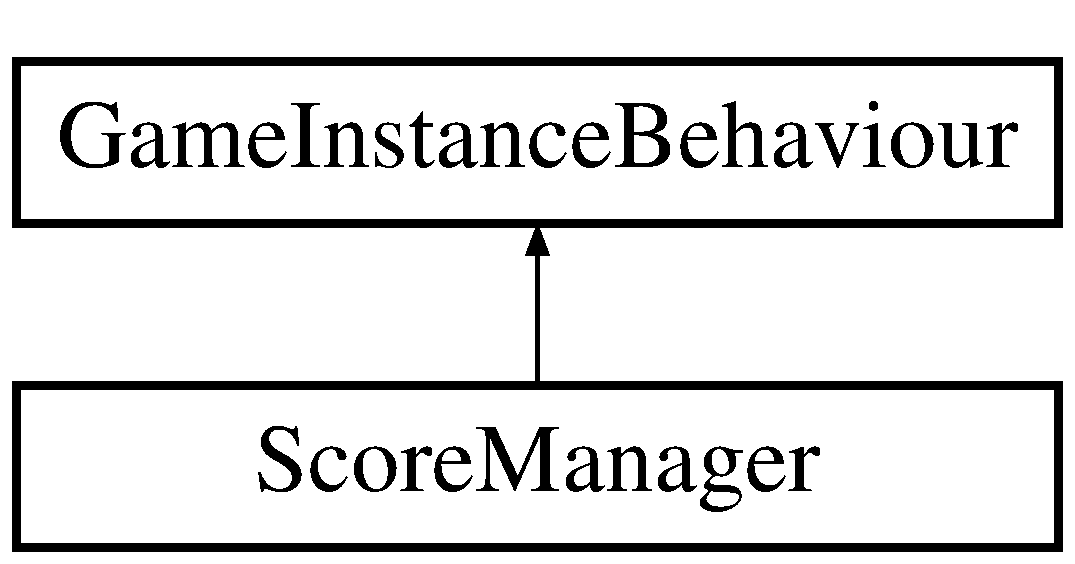
\includegraphics[height=2.000000cm]{class_score_manager}
\end{center}
\end{figure}
\subsection*{Public Member Functions}
\begin{DoxyCompactItemize}
\item 
delegate void {\bfseries On\+Update\+Score} (int score)\hypertarget{class_score_manager_a0d535c5b349c2b0986b13ffcefbbfcd4}{}\label{class_score_manager_a0d535c5b349c2b0986b13ffcefbbfcd4}

\item 
delegate void {\bfseries On\+Update\+Pot} (int pot)\hypertarget{class_score_manager_acf4a27a78b14dcc45d59fbad960335df}{}\label{class_score_manager_acf4a27a78b14dcc45d59fbad960335df}

\item 
void {\bfseries Init} ()\hypertarget{class_score_manager_a5a4a682601029dcffa1bc6a79c78931e}{}\label{class_score_manager_a5a4a682601029dcffa1bc6a79c78931e}

\item 
void \hyperlink{class_score_manager_a2df20bbab8cd763e80b3f6e023552c62}{Fill\+Pot} ()
\begin{DoxyCompactList}\small\item\em Sets the pot to its starting value \end{DoxyCompactList}\item 
void \hyperlink{class_score_manager_a8963c413e2eb854856f32419cb41424a}{Empty\+Pot} ()
\begin{DoxyCompactList}\small\item\em Sets the pot value to 0 \end{DoxyCompactList}\item 
void \hyperlink{class_score_manager_a11408d13d0abff357b56d99324c6037b}{Add\+Round\+Start\+Scores} ()
\begin{DoxyCompactList}\small\item\em Adds coins to each player\textquotesingle{}s score based on what round number this is and whether or not the player is the Decider \end{DoxyCompactList}\item 
void \hyperlink{class_score_manager_addad3c65a8df534fb8d897a9f2b2b3d8}{Add\+Winnings} ()
\begin{DoxyCompactList}\small\item\em Adds coins to the winning player\textquotesingle{}s score \end{DoxyCompactList}\item 
void \hyperlink{class_score_manager_a01d67da43955f99b3715971e5fadce01}{Apply\+Player\+Reward} (Player\+Agenda\+Item item)
\begin{DoxyCompactList}\small\item\em Adds coins to the player\textquotesingle{}s score based on the value defined in the agenda item \end{DoxyCompactList}\end{DoxyCompactItemize}
\subsection*{Public Attributes}
\begin{DoxyCompactItemize}
\item 
On\+Update\+Score \hyperlink{class_score_manager_a54ededdc900a0c1982c25ab9ca984bed}{on\+Update\+Score}
\begin{DoxyCompactList}\small\item\em Event that is called when the player\textquotesingle{}s score is updated. \end{DoxyCompactList}\item 
On\+Update\+Pot \hyperlink{class_score_manager_a2df09d1f61b32b83a80c78d63f94689b}{on\+Update\+Pot}
\begin{DoxyCompactList}\small\item\em Event that is called when the pot\textquotesingle{}s value is updated. \end{DoxyCompactList}\end{DoxyCompactItemize}
\subsection*{Properties}
\begin{DoxyCompactItemize}
\item 
int \hyperlink{class_score_manager_a1a7ae6889437a8e47fac4ca2036149b3}{Player\+Score}\hspace{0.3cm}{\ttfamily  \mbox{[}get, set\mbox{]}}
\begin{DoxyCompactList}\small\item\em Gets/sets this player\textquotesingle{}s score. Sends a notification that the score has been updated. \end{DoxyCompactList}\item 
int \hyperlink{class_score_manager_a4e64c104c582dbe98703bfaa2a6bf196}{Pot}\hspace{0.3cm}{\ttfamily  \mbox{[}get, set\mbox{]}}
\begin{DoxyCompactList}\small\item\em Gets/sets the pot value. Sends a notification that the pot has been updated. \end{DoxyCompactList}\item 
Dictionary$<$ string, int $>$ \hyperlink{class_score_manager_a160ee3a7dbcadcca8a0c623719394681}{Player\+Scores}\hspace{0.3cm}{\ttfamily  \mbox{[}get\mbox{]}}
\begin{DoxyCompactList}\small\item\em Gets the scores for each player. The key is the player\textquotesingle{}s name. \end{DoxyCompactList}\item 
Key\+Value\+Pair$<$ string, int $>$ \hyperlink{class_score_manager_aea653edd704e7a996e77ac55f23a9782}{Top\+Score}\hspace{0.3cm}{\ttfamily  \mbox{[}get\mbox{]}}
\begin{DoxyCompactList}\small\item\em Gets the top score. The key is the player\textquotesingle{}s name. \end{DoxyCompactList}\item 
bool \hyperlink{class_score_manager_a45b9f26bc13807ae1733feea8a5c7349}{Can\+Afford\+Extra\+Time}\hspace{0.3cm}{\ttfamily  \mbox{[}get\mbox{]}}
\begin{DoxyCompactList}\small\item\em Returns true if the player\textquotesingle{}s score is large enough to be able to afford extra time. \end{DoxyCompactList}\end{DoxyCompactItemize}


\subsection{Detailed Description}
Interfaces with Game\+Controller to handle scoring for all players This includes players\textquotesingle{} individual scores and the pot 



\subsection{Member Function Documentation}
\index{Score\+Manager@{Score\+Manager}!Add\+Round\+Start\+Scores@{Add\+Round\+Start\+Scores}}
\index{Add\+Round\+Start\+Scores@{Add\+Round\+Start\+Scores}!Score\+Manager@{Score\+Manager}}
\subsubsection[{\texorpdfstring{Add\+Round\+Start\+Scores()}{AddRoundStartScores()}}]{\setlength{\rightskip}{0pt plus 5cm}void Score\+Manager.\+Add\+Round\+Start\+Scores (
\begin{DoxyParamCaption}
{}
\end{DoxyParamCaption}
)}\hypertarget{class_score_manager_a11408d13d0abff357b56d99324c6037b}{}\label{class_score_manager_a11408d13d0abff357b56d99324c6037b}


Adds coins to each player\textquotesingle{}s score based on what round number this is and whether or not the player is the Decider 

\index{Score\+Manager@{Score\+Manager}!Add\+Winnings@{Add\+Winnings}}
\index{Add\+Winnings@{Add\+Winnings}!Score\+Manager@{Score\+Manager}}
\subsubsection[{\texorpdfstring{Add\+Winnings()}{AddWinnings()}}]{\setlength{\rightskip}{0pt plus 5cm}void Score\+Manager.\+Add\+Winnings (
\begin{DoxyParamCaption}
{}
\end{DoxyParamCaption}
)}\hypertarget{class_score_manager_addad3c65a8df534fb8d897a9f2b2b3d8}{}\label{class_score_manager_addad3c65a8df534fb8d897a9f2b2b3d8}


Adds coins to the winning player\textquotesingle{}s score 

\index{Score\+Manager@{Score\+Manager}!Apply\+Player\+Reward@{Apply\+Player\+Reward}}
\index{Apply\+Player\+Reward@{Apply\+Player\+Reward}!Score\+Manager@{Score\+Manager}}
\subsubsection[{\texorpdfstring{Apply\+Player\+Reward(\+Player\+Agenda\+Item item)}{ApplyPlayerReward(PlayerAgendaItem item)}}]{\setlength{\rightskip}{0pt plus 5cm}void Score\+Manager.\+Apply\+Player\+Reward (
\begin{DoxyParamCaption}
\item[{Player\+Agenda\+Item}]{item}
\end{DoxyParamCaption}
)}\hypertarget{class_score_manager_a01d67da43955f99b3715971e5fadce01}{}\label{class_score_manager_a01d67da43955f99b3715971e5fadce01}


Adds coins to the player\textquotesingle{}s score based on the value defined in the agenda item 

\index{Score\+Manager@{Score\+Manager}!Empty\+Pot@{Empty\+Pot}}
\index{Empty\+Pot@{Empty\+Pot}!Score\+Manager@{Score\+Manager}}
\subsubsection[{\texorpdfstring{Empty\+Pot()}{EmptyPot()}}]{\setlength{\rightskip}{0pt plus 5cm}void Score\+Manager.\+Empty\+Pot (
\begin{DoxyParamCaption}
{}
\end{DoxyParamCaption}
)}\hypertarget{class_score_manager_a8963c413e2eb854856f32419cb41424a}{}\label{class_score_manager_a8963c413e2eb854856f32419cb41424a}


Sets the pot value to 0 

\index{Score\+Manager@{Score\+Manager}!Fill\+Pot@{Fill\+Pot}}
\index{Fill\+Pot@{Fill\+Pot}!Score\+Manager@{Score\+Manager}}
\subsubsection[{\texorpdfstring{Fill\+Pot()}{FillPot()}}]{\setlength{\rightskip}{0pt plus 5cm}void Score\+Manager.\+Fill\+Pot (
\begin{DoxyParamCaption}
{}
\end{DoxyParamCaption}
)}\hypertarget{class_score_manager_a2df20bbab8cd763e80b3f6e023552c62}{}\label{class_score_manager_a2df20bbab8cd763e80b3f6e023552c62}


Sets the pot to its starting value 



\subsection{Member Data Documentation}
\index{Score\+Manager@{Score\+Manager}!on\+Update\+Pot@{on\+Update\+Pot}}
\index{on\+Update\+Pot@{on\+Update\+Pot}!Score\+Manager@{Score\+Manager}}
\subsubsection[{\texorpdfstring{on\+Update\+Pot}{onUpdatePot}}]{\setlength{\rightskip}{0pt plus 5cm}On\+Update\+Pot Score\+Manager.\+on\+Update\+Pot}\hypertarget{class_score_manager_a2df09d1f61b32b83a80c78d63f94689b}{}\label{class_score_manager_a2df09d1f61b32b83a80c78d63f94689b}


Event that is called when the pot\textquotesingle{}s value is updated. 

\index{Score\+Manager@{Score\+Manager}!on\+Update\+Score@{on\+Update\+Score}}
\index{on\+Update\+Score@{on\+Update\+Score}!Score\+Manager@{Score\+Manager}}
\subsubsection[{\texorpdfstring{on\+Update\+Score}{onUpdateScore}}]{\setlength{\rightskip}{0pt plus 5cm}On\+Update\+Score Score\+Manager.\+on\+Update\+Score}\hypertarget{class_score_manager_a54ededdc900a0c1982c25ab9ca984bed}{}\label{class_score_manager_a54ededdc900a0c1982c25ab9ca984bed}


Event that is called when the player\textquotesingle{}s score is updated. 



\subsection{Property Documentation}
\index{Score\+Manager@{Score\+Manager}!Can\+Afford\+Extra\+Time@{Can\+Afford\+Extra\+Time}}
\index{Can\+Afford\+Extra\+Time@{Can\+Afford\+Extra\+Time}!Score\+Manager@{Score\+Manager}}
\subsubsection[{\texorpdfstring{Can\+Afford\+Extra\+Time}{CanAffordExtraTime}}]{\setlength{\rightskip}{0pt plus 5cm}bool Score\+Manager.\+Can\+Afford\+Extra\+Time\hspace{0.3cm}{\ttfamily [get]}}\hypertarget{class_score_manager_a45b9f26bc13807ae1733feea8a5c7349}{}\label{class_score_manager_a45b9f26bc13807ae1733feea8a5c7349}


Returns true if the player\textquotesingle{}s score is large enough to be able to afford extra time. 

\index{Score\+Manager@{Score\+Manager}!Player\+Score@{Player\+Score}}
\index{Player\+Score@{Player\+Score}!Score\+Manager@{Score\+Manager}}
\subsubsection[{\texorpdfstring{Player\+Score}{PlayerScore}}]{\setlength{\rightskip}{0pt plus 5cm}int Score\+Manager.\+Player\+Score\hspace{0.3cm}{\ttfamily [get]}, {\ttfamily [set]}}\hypertarget{class_score_manager_a1a7ae6889437a8e47fac4ca2036149b3}{}\label{class_score_manager_a1a7ae6889437a8e47fac4ca2036149b3}


Gets/sets this player\textquotesingle{}s score. Sends a notification that the score has been updated. 

\index{Score\+Manager@{Score\+Manager}!Player\+Scores@{Player\+Scores}}
\index{Player\+Scores@{Player\+Scores}!Score\+Manager@{Score\+Manager}}
\subsubsection[{\texorpdfstring{Player\+Scores}{PlayerScores}}]{\setlength{\rightskip}{0pt plus 5cm}Dictionary$<$string, int$>$ Score\+Manager.\+Player\+Scores\hspace{0.3cm}{\ttfamily [get]}}\hypertarget{class_score_manager_a160ee3a7dbcadcca8a0c623719394681}{}\label{class_score_manager_a160ee3a7dbcadcca8a0c623719394681}


Gets the scores for each player. The key is the player\textquotesingle{}s name. 

\index{Score\+Manager@{Score\+Manager}!Pot@{Pot}}
\index{Pot@{Pot}!Score\+Manager@{Score\+Manager}}
\subsubsection[{\texorpdfstring{Pot}{Pot}}]{\setlength{\rightskip}{0pt plus 5cm}int Score\+Manager.\+Pot\hspace{0.3cm}{\ttfamily [get]}, {\ttfamily [set]}}\hypertarget{class_score_manager_a4e64c104c582dbe98703bfaa2a6bf196}{}\label{class_score_manager_a4e64c104c582dbe98703bfaa2a6bf196}


Gets/sets the pot value. Sends a notification that the pot has been updated. 

\index{Score\+Manager@{Score\+Manager}!Top\+Score@{Top\+Score}}
\index{Top\+Score@{Top\+Score}!Score\+Manager@{Score\+Manager}}
\subsubsection[{\texorpdfstring{Top\+Score}{TopScore}}]{\setlength{\rightskip}{0pt plus 5cm}Key\+Value\+Pair$<$string, int$>$ Score\+Manager.\+Top\+Score\hspace{0.3cm}{\ttfamily [get]}}\hypertarget{class_score_manager_aea653edd704e7a996e77ac55f23a9782}{}\label{class_score_manager_aea653edd704e7a996e77ac55f23a9782}


Gets the top score. The key is the player\textquotesingle{}s name. 



The documentation for this class was generated from the following file\+:\begin{DoxyCompactItemize}
\item 
Assets/\+Scripts/Score\+Manager.\+cs\end{DoxyCompactItemize}

%--- End generated contents ---

% Index
\backmatter
\newpage
\phantomsection
\clearemptydoublepage
\addcontentsline{toc}{chapter}{Index}
\printindex

\end{document}
